% Options for packages loaded elsewhere
\PassOptionsToPackage{unicode}{hyperref}
\PassOptionsToPackage{hyphens}{url}
\PassOptionsToPackage{dvipsnames,svgnames,x11names}{xcolor}
%
\documentclass[
  letterpaper,
  DIV=11,
  numbers=noendperiod]{scrartcl}

\usepackage{amsmath,amssymb}
\usepackage{iftex}
\ifPDFTeX
  \usepackage[T1]{fontenc}
  \usepackage[utf8]{inputenc}
  \usepackage{textcomp} % provide euro and other symbols
\else % if luatex or xetex
  \usepackage{unicode-math}
  \defaultfontfeatures{Scale=MatchLowercase}
  \defaultfontfeatures[\rmfamily]{Ligatures=TeX,Scale=1}
\fi
\usepackage{lmodern}
\ifPDFTeX\else  
    % xetex/luatex font selection
\fi
% Use upquote if available, for straight quotes in verbatim environments
\IfFileExists{upquote.sty}{\usepackage{upquote}}{}
\IfFileExists{microtype.sty}{% use microtype if available
  \usepackage[]{microtype}
  \UseMicrotypeSet[protrusion]{basicmath} % disable protrusion for tt fonts
}{}
\makeatletter
\@ifundefined{KOMAClassName}{% if non-KOMA class
  \IfFileExists{parskip.sty}{%
    \usepackage{parskip}
  }{% else
    \setlength{\parindent}{0pt}
    \setlength{\parskip}{6pt plus 2pt minus 1pt}}
}{% if KOMA class
  \KOMAoptions{parskip=half}}
\makeatother
\usepackage{xcolor}
\setlength{\emergencystretch}{3em} % prevent overfull lines
\setcounter{secnumdepth}{5}
% Make \paragraph and \subparagraph free-standing
\ifx\paragraph\undefined\else
  \let\oldparagraph\paragraph
  \renewcommand{\paragraph}[1]{\oldparagraph{#1}\mbox{}}
\fi
\ifx\subparagraph\undefined\else
  \let\oldsubparagraph\subparagraph
  \renewcommand{\subparagraph}[1]{\oldsubparagraph{#1}\mbox{}}
\fi


\providecommand{\tightlist}{%
  \setlength{\itemsep}{0pt}\setlength{\parskip}{0pt}}\usepackage{longtable,booktabs,array}
\usepackage{calc} % for calculating minipage widths
% Correct order of tables after \paragraph or \subparagraph
\usepackage{etoolbox}
\makeatletter
\patchcmd\longtable{\par}{\if@noskipsec\mbox{}\fi\par}{}{}
\makeatother
% Allow footnotes in longtable head/foot
\IfFileExists{footnotehyper.sty}{\usepackage{footnotehyper}}{\usepackage{footnote}}
\makesavenoteenv{longtable}
\usepackage{graphicx}
\makeatletter
\def\maxwidth{\ifdim\Gin@nat@width>\linewidth\linewidth\else\Gin@nat@width\fi}
\def\maxheight{\ifdim\Gin@nat@height>\textheight\textheight\else\Gin@nat@height\fi}
\makeatother
% Scale images if necessary, so that they will not overflow the page
% margins by default, and it is still possible to overwrite the defaults
% using explicit options in \includegraphics[width, height, ...]{}
\setkeys{Gin}{width=\maxwidth,height=\maxheight,keepaspectratio}
% Set default figure placement to htbp
\makeatletter
\def\fps@figure{htbp}
\makeatother
\newlength{\cslhangindent}
\setlength{\cslhangindent}{1.5em}
\newlength{\csllabelwidth}
\setlength{\csllabelwidth}{3em}
\newlength{\cslentryspacingunit} % times entry-spacing
\setlength{\cslentryspacingunit}{\parskip}
\newenvironment{CSLReferences}[2] % #1 hanging-ident, #2 entry spacing
 {% don't indent paragraphs
  \setlength{\parindent}{0pt}
  % turn on hanging indent if param 1 is 1
  \ifodd #1
  \let\oldpar\par
  \def\par{\hangindent=\cslhangindent\oldpar}
  \fi
  % set entry spacing
  \setlength{\parskip}{#2\cslentryspacingunit}
 }%
 {}
\usepackage{calc}
\newcommand{\CSLBlock}[1]{#1\hfill\break}
\newcommand{\CSLLeftMargin}[1]{\parbox[t]{\csllabelwidth}{#1}}
\newcommand{\CSLRightInline}[1]{\parbox[t]{\linewidth - \csllabelwidth}{#1}\break}
\newcommand{\CSLIndent}[1]{\hspace{\cslhangindent}#1}

\usepackage{booktabs}
\usepackage{longtable}
\usepackage{array}
\usepackage{multirow}
\usepackage{wrapfig}
\usepackage{float}
\usepackage{colortbl}
\usepackage{pdflscape}
\usepackage{tabu}
\usepackage{threeparttable}
\usepackage{threeparttablex}
\usepackage[normalem]{ulem}
\usepackage{makecell}
\usepackage{xcolor}
\KOMAoption{captions}{tableheading}
\makeatletter
\makeatother
\makeatletter
\makeatother
\makeatletter
\@ifpackageloaded{caption}{}{\usepackage{caption}}
\AtBeginDocument{%
\ifdefined\contentsname
  \renewcommand*\contentsname{Table of contents}
\else
  \newcommand\contentsname{Table of contents}
\fi
\ifdefined\listfigurename
  \renewcommand*\listfigurename{List of Figures}
\else
  \newcommand\listfigurename{List of Figures}
\fi
\ifdefined\listtablename
  \renewcommand*\listtablename{List of Tables}
\else
  \newcommand\listtablename{List of Tables}
\fi
\ifdefined\figurename
  \renewcommand*\figurename{Figure}
\else
  \newcommand\figurename{Figure}
\fi
\ifdefined\tablename
  \renewcommand*\tablename{Table}
\else
  \newcommand\tablename{Table}
\fi
}
\@ifpackageloaded{float}{}{\usepackage{float}}
\floatstyle{ruled}
\@ifundefined{c@chapter}{\newfloat{codelisting}{h}{lop}}{\newfloat{codelisting}{h}{lop}[chapter]}
\floatname{codelisting}{Listing}
\newcommand*\listoflistings{\listof{codelisting}{List of Listings}}
\makeatother
\makeatletter
\@ifpackageloaded{caption}{}{\usepackage{caption}}
\@ifpackageloaded{subcaption}{}{\usepackage{subcaption}}
\makeatother
\makeatletter
\@ifpackageloaded{tcolorbox}{}{\usepackage[skins,breakable]{tcolorbox}}
\makeatother
\makeatletter
\@ifundefined{shadecolor}{\definecolor{shadecolor}{rgb}{.97, .97, .97}}
\makeatother
\makeatletter
\makeatother
\makeatletter
\makeatother
\ifLuaTeX
  \usepackage{selnolig}  % disable illegal ligatures
\fi
\IfFileExists{bookmark.sty}{\usepackage{bookmark}}{\usepackage{hyperref}}
\IfFileExists{xurl.sty}{\usepackage{xurl}}{} % add URL line breaks if available
\urlstyle{same} % disable monospaced font for URLs
\hypersetup{
  pdftitle={My title},
  pdfauthor={First author; Another author},
  colorlinks=true,
  linkcolor={blue},
  filecolor={Maroon},
  citecolor={Blue},
  urlcolor={Blue},
  pdfcreator={LaTeX via pandoc}}

\title{My title\thanks{Code and data are available at: LINK.}}
\usepackage{etoolbox}
\makeatletter
\providecommand{\subtitle}[1]{% add subtitle to \maketitle
  \apptocmd{\@title}{\par {\large #1 \par}}{}{}
}
\makeatother
\subtitle{My subtitle if needed}
\author{First author \and Another author}
\date{March 19, 2024}

\begin{document}
\maketitle
\begin{abstract}
First sentence. Second sentence. Third sentence. Fourth sentence.
\end{abstract}
\ifdefined\Shaded\renewenvironment{Shaded}{\begin{tcolorbox}[frame hidden, boxrule=0pt, interior hidden, sharp corners, breakable, enhanced, borderline west={3pt}{0pt}{shadecolor}]}{\end{tcolorbox}}\fi

\begin{verbatim}

Attaching package: 'kableExtra'
\end{verbatim}

\begin{verbatim}
The following object is masked from 'package:dplyr':

    group_rows
\end{verbatim}

\begin{table}
\centering
\begin{tabular}[t]{l|l}
\hline
variables & observations\\
\hline
All Americans & All the following groups\\
\hline
Race & Self-identified race of participants\\
\hline
Gender & Male/Female\\
\hline
Political Affiliation & Democrat/Republican/Other\\
\hline
Level of Education & College Degree or Higher/Highschool Diploma/No Highschool Diploma\\
\hline
\end{tabular}
\end{table}

\hypertarget{introduction}{%
\section{Introduction}\label{introduction}}

You can and should cross-reference sections and sub-sections. We use R
Core Team (2023) and Wickham et al. (2019).

The remainder of this paper is structured as follows.
Section~\ref{sec-data}\ldots.

\hypertarget{sec-data}{%
\section{Data}\label{sec-data}}

//sum up gen survey and the questions the survey is intended to ask.
Background about the GSS.

Background about the sampling methodology

Background about the questions that are asked.

Plot each variable of interest and add discussion around them.

Talk more about it.

(You can change the height and width, but don't worry about doing that
until you have finished every other aspect of the paper - Quarto will
try to make it look nice and the defaults usually work well once you
have enough text.)

Talk way more about it.

\hypertarget{results}{%
\section{Results}\label{results}}

Our results are summarized in.

//Add some analysis here. So that might be looking at difference over
time or between states or between genders. Whatever.

When looking at a general overview regarding sentiment towards mandatory
gun permits for firearm owners in the United States, it's clear that in
more recent years there has been less support for citizens having
permits. Support for mandatory gun permits increased under the Reagan
Republican administration. Support for mandatory gun permits started to
decrease around the time of 2001/02. From 2002 onward sentiment toward
mandatory gun permits has steadily decreased regardless of which party
controlled the White House. Even during the Democratic party's Obama
administration support for mandatory gun permits decreased.

//Graph of the total//

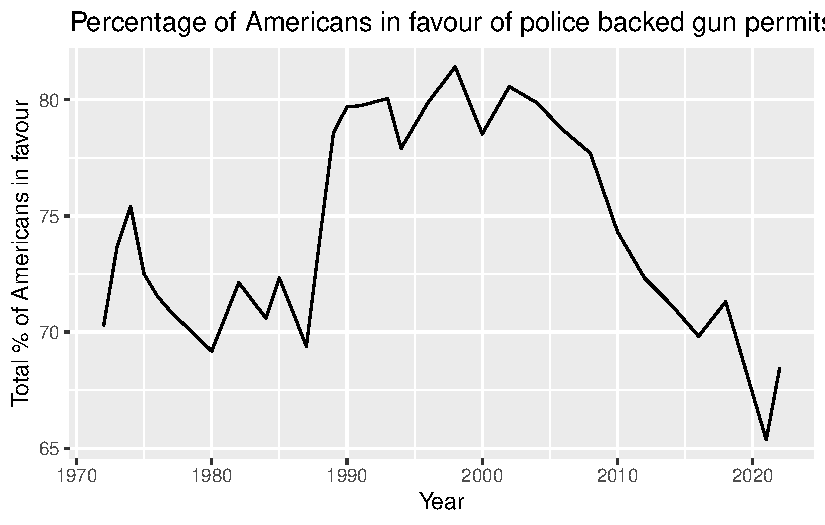
\includegraphics{paper_files/figure-pdf/unnamed-chunk-5-1.pdf}

Looking at how sentiments differ between Republicans and Democrats is
also noteworthy. The second term of the George W. Bush Administration in
2004 Is notable as the starting point for when sentiments towards
mandatory gun permit ownership became more polarizing. While the views
of voting Democrats remain pretty consistent, the views of Republicans
start to differ going forward into the following administrations from
where they were under the previous Clinton administration. Before the
George W Bush administration, sentiments differed, but were similar
between both Republican- and Democrat-voting Americans.

//Graph of DEMS VS REPUBLICANS//

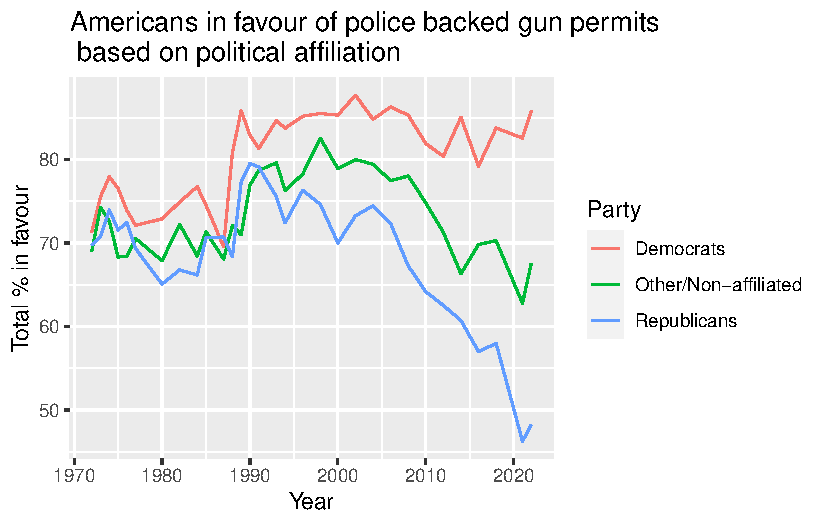
\includegraphics{paper_files/figure-pdf/unnamed-chunk-6-1.pdf}

Additionally worth note is how sentiments towards gun permits change
depending on Americans' level of Education. Those with a college degree
or higher overall have greater support towards gun owners having a
permit, followed by Americans without high school diplomas. The lowest
support for gun owners requiring permits comes from Americans that have
a high school diploma and no college degree.

//Graph of Education level and opinions for gun permits

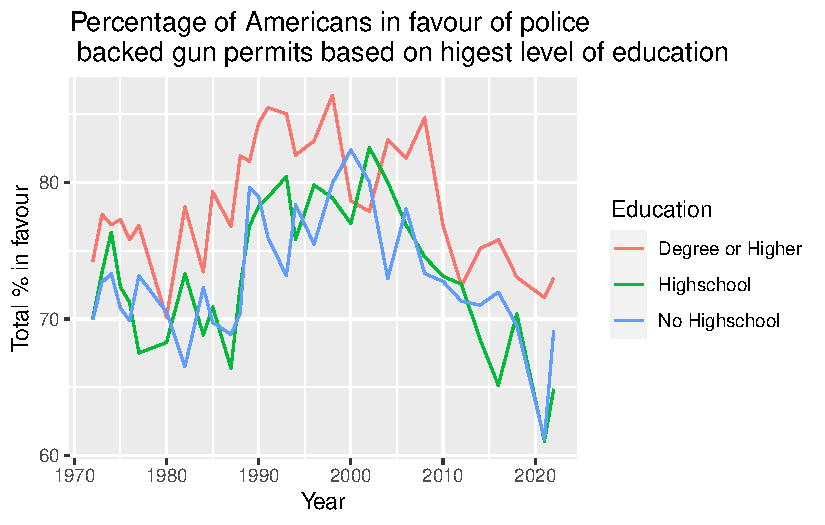
\includegraphics{paper_files/figure-pdf/unnamed-chunk-7-1.pdf}

We can also observe a large difference between male and female opinions
on gun permits, where there is a consistent 15-20\% difference towards
mandatory enforcement of gun permits.

//Graph of MaleVsFemale

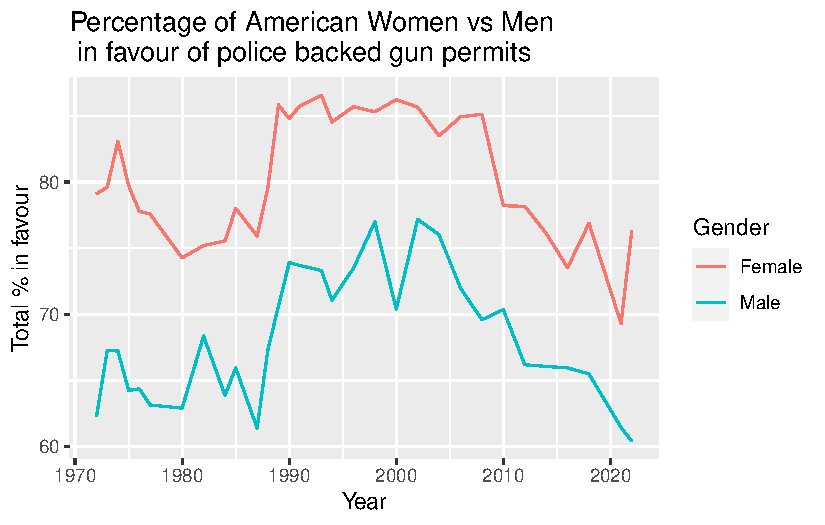
\includegraphics{paper_files/figure-pdf/unnamed-chunk-8-1.pdf}

Race also appears to interact with gun ownership sentiments. Almost
consistently, white people are less in favour of police backed mandatory
gun permits. However, the omission of other racial groups in favour of
one group called ``other'' makes it difficult to get a sense for the
true opinions of America based on race. By combining many groups into
one, we can observe a very volatile line on the graph that jumps between
extremes multiple times before 1989. This data collection choice makes
interpretation and comprehension difficult.

///Graph of Race and Gun Law

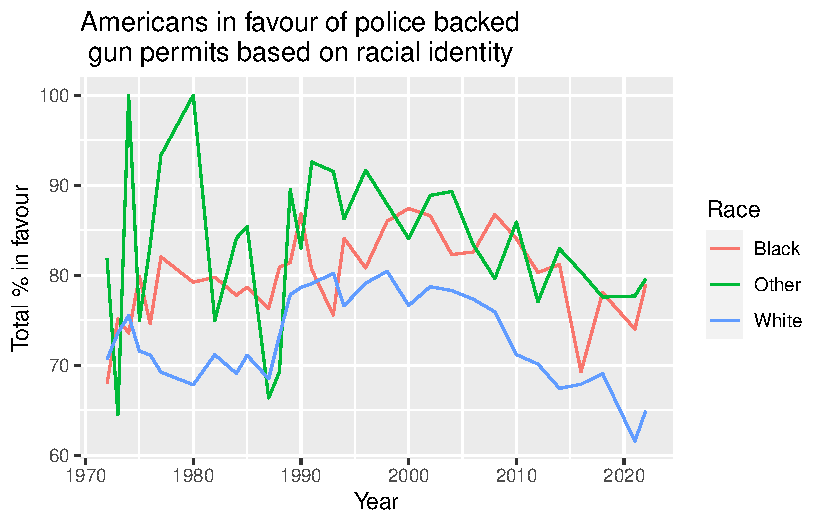
\includegraphics{paper_files/figure-pdf/unnamed-chunk-9-1.pdf}

\hypertarget{discussion}{%
\section{Discussion}\label{discussion}}

\hypertarget{sec-first-point}{%
\subsection{First discussion point}\label{sec-first-point}}

If my paper were 10 pages, then should be be at least 2.5 pages. The
discussion is a chance to show off what you know and what you learnt
from all this.

\hypertarget{second-discussion-point}{%
\subsection{Second discussion point}\label{second-discussion-point}}

\hypertarget{third-discussion-point}{%
\subsection{Third discussion point}\label{third-discussion-point}}

\hypertarget{weaknesses-and-next-steps}{%
\subsection{Weaknesses and next steps}\label{weaknesses-and-next-steps}}

Weaknesses and next steps should also be included.

\newpage

\appendix

\hypertarget{appendix}{%
\section*{Appendix}\label{appendix}}
\addcontentsline{toc}{section}{Appendix}

\hypertarget{references}{%
\section*{References}\label{references}}
\addcontentsline{toc}{section}{References}

\hypertarget{refs}{}
\begin{CSLReferences}{1}{0}
\leavevmode\vadjust pre{\hypertarget{ref-citeR}{}}%
R Core Team. 2023. \emph{R: A Language and Environment for Statistical
Computing}. Vienna, Austria: R Foundation for Statistical Computing.
\url{https://www.R-project.org/}.

\leavevmode\vadjust pre{\hypertarget{ref-rohan}{}}%
Wickham, Hadley, Mara Averick, Jennifer Bryan, Winston Chang, Lucy
D'Agostino McGowan, Romain François, Garrett Grolemund, et al. 2019.
{``Welcome to the {tidyverse}.''} \emph{Journal of Open Source Software}
4 (43): 1686. \url{https://doi.org/10.21105/joss.01686}.

\end{CSLReferences}



\end{document}
